\begin{figure}[H]
	\centering
	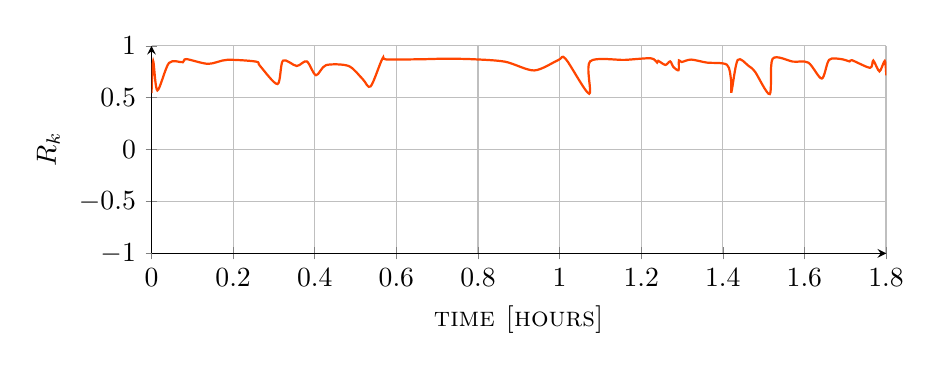
\begin{tikzpicture}
		\begin{axis}[xlabel=\textsc{time [hours]}, ylabel=\textsc{$R_k$}, axis lines=left, grid=major, width=0.9\linewidth, height=12em, ymax=1, ymin=-1]
			\addplot +[mark=none, OrangeRed, thick, smooth] table {
				0.0 0.5444961087808939
				0.004123611111111111 0.8511537523863583
				0.014372777777777778 0.5698992049269191
				0.04273444444444444 0.8343897290417408
				0.0768911111111111 0.8420760152871233
				0.08518444444444444 0.8720495595978613
				0.1388125 0.8261894646121312
				0.1851913888888889 0.8647541227129498
				0.2556111111111111 0.8480853222797268
				0.2658975 0.8060343441693703
				0.30876583333333335 0.6314028702965143
				0.32202416666666667 0.8571194077490936
				0.35565861111111113 0.8056351236685689
				0.3804983333333334 0.8500353157544382
				0.40297805555555555 0.7166104670945992
				0.4277680555555555 0.8138154044494291
				0.4829122222222222 0.8057550379098798
				0.51748 0.6794566906676353
				0.5370322222222222 0.6090771980973686
				0.5658177777777778 0.8761208672966857
				0.576466111111111 0.8672553755060747
				0.661583888888889 0.8705752127728053
				0.7201791666666667 0.8756231672197796
				0.7876677777777777 0.8707195219011391
				0.8665727777777777 0.8467565915633849
				0.9376275 0.7627236065746218
				0.9966172222222223 0.862060541044936
				1.0146355555555555 0.8752327058794888
				1.072577222222222 0.5382420926474235
				1.0748411111111111 0.8500503513023147
				1.1602050000000002 0.8644253104569336
				1.2235383333333334 0.8796329750244695
				1.2390402777777778 0.8385568338949455
				1.2416858333333334 0.8552891635030724
				1.2592969444444444 0.8158802457284906
				1.2711222222222223 0.8507323159260161
				1.2781972222222222 0.7998536171046322
				1.2914630555555555 0.7643073894042848
				1.2925022222222222 0.859163337005119
				1.2991336111111111 0.8438732544884482
				1.3223772222222223 0.8673012928378777
				1.3605297222222223 0.8384795432300679
				1.410015277777778 0.8179457028540305
				1.420321388888889 0.6643935940130762
				1.4213269444444445 0.5576689836005811
				1.436411388888889 0.8633325091985307
				1.4630463888888887 0.8069793168229261
				1.4794466666666666 0.747253453002513
				1.5151569444444444 0.5348611407238524
				1.5221622222222222 0.8751174506904024
				1.5722874999999998 0.847666981150265
				1.6098002777777778 0.8372189474100846
				1.6425980555555555 0.6849397502111092
				1.6605197222222223 0.8644031385554191
				1.6898397222222221 0.8721161602009476
				1.7107966666666667 0.8497743934293334
				1.716603888888889 0.8612318359681981
				1.7608688888888888 0.7879840626524268
				1.7688858333333333 0.8577422363343189
				1.783848611111111 0.7537154075635912
				1.796906111111111 0.8538259300513192
				1.800613611111111 0.71603006988279
			};
		\end{axis}
	\end{tikzpicture}
	\caption{Hyper-parameters optimization plot for the category classifier based on random forest.}
	\label{fig:optimization_category_random_forest}
\end{figure}
\begin{table}[H]
	\centering
	\begin{tabular}{ll}
		\toprule
		\textsc{hyper-parameter} & \textsc{value}\\
		\midrule
		\verb|criterion| & entropy\\
		\verb|max_depth| & 17\\
		\verb|min_samples_leaf| & 9\\
		\verb|min_samples_split| & 38\\
		\verb|n_estimators| & 89\\
		\bottomrule
	\end{tabular}
	\caption{Optimal hyper-parameters for the category classifier based on random forest.}
	\label{tab:hyperparameters_category_random_forest}
\end{table}
\begin{table}[H]
	\centering
	\begin{tabular}{lrrrr}
		\toprule
		\textsc{statistic} & \textsc{training set} & \textsc{dev set} & \textsc{kts} & \textsc{uts}\\
		\midrule
		samples & 955872 & 119484 & 119485 & 30144\\
		accuracy [$\%$] & 97.702 & 97.542 & 97.447 & 40.459\\
		balanced accuracy [$\%$] & 95.568 & 93.997 & 94.041 & 34.031\\
		precision [$\%$] & 86.660 & 85.637 & 85.226 & 32.723\\
		recall [$\%$] & 95.568 & 93.997 & 94.041 & 34.031\\
		Cohen’s kappa [$\%$] & 86.105 & 85.021 & 84.577 & 1.097\\
		F-score [$\%$] & 90.719 & 89.459 & 89.230 & 32.151\\
		Jaccard score [$\%$] & 83.556 & 81.607 & 81.255 & 20.631\\
		Hamming loss & 0.023 & 0.025 & 0.026 & 0.595\\
		zero-one loss & 0.023 & 0.025 & 0.026 & 0.595\\
		$R_k$ & 0.865 & 0.854 & 0.850 & 0.011\\
		\bottomrule
	\end{tabular}
	\caption{Classification statistics for the category classifier based on random forest.}
	\label{tab:classification_category_random_forest}
\end{table}
\begin{table}[H]
	\centering
	\begin{tabular}{ll|lll}
	\setlength{\tabcolsep}{2pt}
		 & & \multicolumn{3}{c}{\textsc{inferred}}\\
		 & & \textsc{browser} & \textsc{crawler} & \textsc{dos}\\
		\midrule
		\multirow{3}{*}{\rotatebox{90}{\textsc{target}}} & \textsc{browser} & 6872 & 194 & 322\\
		 & \textsc{crawler} & 120 & 2112 & 83\\
		 & \textsc{dos} & 1980 & 352 & 107450\\
	\end{tabular}
	\caption{Confusion matrix for the category classifier based on random forest on the KTS.}
	\label{tab:confusion_category_random_forest}
\end{table}
\begin{figure}[H]
	\centering
	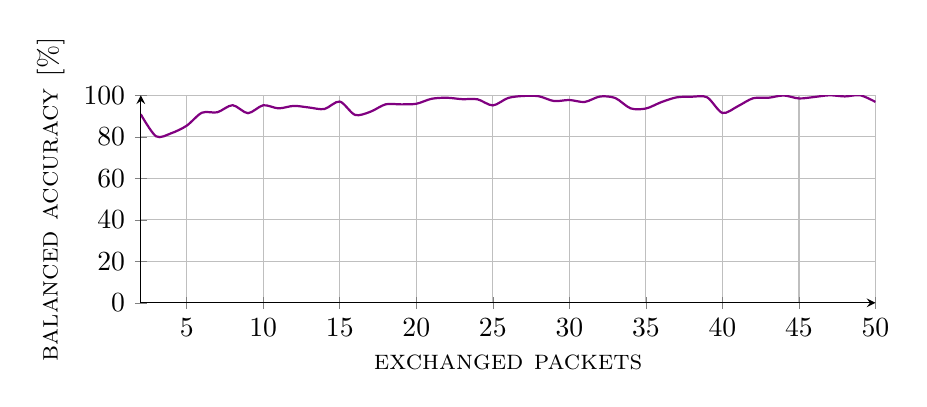
\begin{tikzpicture}
		\begin{axis}[xlabel=\textsc{exchanged packets}, ylabel=\textsc{balanced accuracy [$\%$]}, axis lines=left, grid=major, width=0.9\linewidth, height=12em, ymax=100, ymin=0]
			\addplot +[mark=none, Purple, thick, smooth] table {
				2.0 90.8437826541275
				3.0 80.22175923387613
				4.0 81.73344753465695
				5.0 85.34596811183296
				6.0 91.61303468636976
				7.0 91.80203057112627
				8.0 95.22640971038501
				9.0 91.36070369341854
				10.0 95.18327396668766
				11.0 93.69135587802938
				12.0 94.88908595630309
				13.0 94.09857175822907
				14.0 93.38543917982406
				15.0 96.98121997025248
				16.0 90.53792623521225
				17.0 92.05342784456396
				18.0 95.64432518427675
				19.0 95.61846816545979
				20.0 95.89701398185333
				21.0 98.31200657023261
				22.0 98.80517842038108
				23.0 98.12352459411284
				24.0 98.05082070707071
				25.0 95.12037669932405
				26.0 98.70064967516242
				27.0 99.66996699669967
				28.0 99.53569680441929
				29.0 97.21638655462185
				30.0 97.72358218649778
				31.0 96.77767052767052
				32.0 99.41117240171614
				33.0 98.6711395433505
				34.0 93.70096697682904
				35.0 93.62114076399791
				36.0 96.66879445442113
				37.0 98.98848428260193
				38.0 99.30555555555554
				39.0 99.0135468396338
				40.0 91.4850136239782
				41.0 94.70026727758687
				42.0 98.55776306107433
				43.0 98.79120879120879
				44.0 99.89451476793249
				45.0 98.4729064039409
				46.0 99.16666666666667
				47.0 100.0
				48.0 99.4413407821229
				49.0 100.0
				50.0 96.79633867276888
			};
		\end{axis}
	\end{tikzpicture}
	\caption{Balanced accuracy vs. exchange packets plot for the category classifier based on random forest on the KTS.}
	\label{fig:packets_category_random_forest}
\end{figure}
\begin{table}[H]
	\centering
	\begin{subtable}{.45\linewidth}
		\centering
	\begin{tabular}{ll}
		\toprule
		\textsc{inferred class} & \textsc{samples}\\
		\midrule
		browser & 3291\\
		crawler & 2623\\
		dos & 620\\
		\bottomrule
	\end{tabular}
	\caption{Classification of \textsc{firefox-68.0}.}
	\end{subtable}
	\begin{subtable}{.45\linewidth}
		\centering
	\begin{tabular}{ll}
		\toprule
		\textsc{inferred class} & \textsc{samples}\\
		\midrule
		browser & 1369\\
		crawler & 883\\
		dos & 1413\\
		\bottomrule
	\end{tabular}
	\caption{Classification of \textsc{grabsite-2.1.16}.}
	\end{subtable}
	\begin{subtable}{.45\linewidth}
		\centering
	\begin{tabular}{ll}
		\toprule
		\textsc{inferred class} & \textsc{samples}\\
		\midrule
		browser & 6149\\
		crawler & 605\\
		dos & 2196\\
		\bottomrule
	\end{tabular}
	\caption{Classification of \textsc{opera-62.0.3331.66}.}
	\end{subtable}
	\begin{subtable}{.45\linewidth}
		\centering
	\begin{tabular}{ll}
		\toprule
		\textsc{inferred class} & \textsc{samples}\\
		\midrule
		browser & 6657\\
		crawler & 2465\\
		dos & 1873\\
		\bottomrule
	\end{tabular}
	\caption{Classification of \textsc{slowhttptest-1.6}.}
	\end{subtable}
	\caption{Classification of unknown tools for the category classifier based on random forest.}
	\label{tab:unknown_category_random_forest}
\end{table}
